\subsection{CRUD}

As outlined in the planning for this sprint, the main focus of this sprint was to implement API endpoints for the database.
As we already had a working database, the goal of this increment was to write a CRUD API in C\# that the other layers could use to access the database via HTTP requests.
The CRUD operations we implemented are based on requests from the other layers, and what they believed they needed to retrieve from the database.
To implement this, we split the CRUD operations into three different routes, respectively named: WordCount, WordRatio, and Schema. Each route has its own endpoints and can access different tables in the database. WordCount is used for inserting and querying articles in the database, WordRatio is used as an abstraction over the WordRatio view in the database, and the Schema route is used to insert and query JSON Schemas in the database.

An overview of the components in the API is outlined in figure \ref{Node02Sprint3}.

\begin{figure}[h]
    \centering
    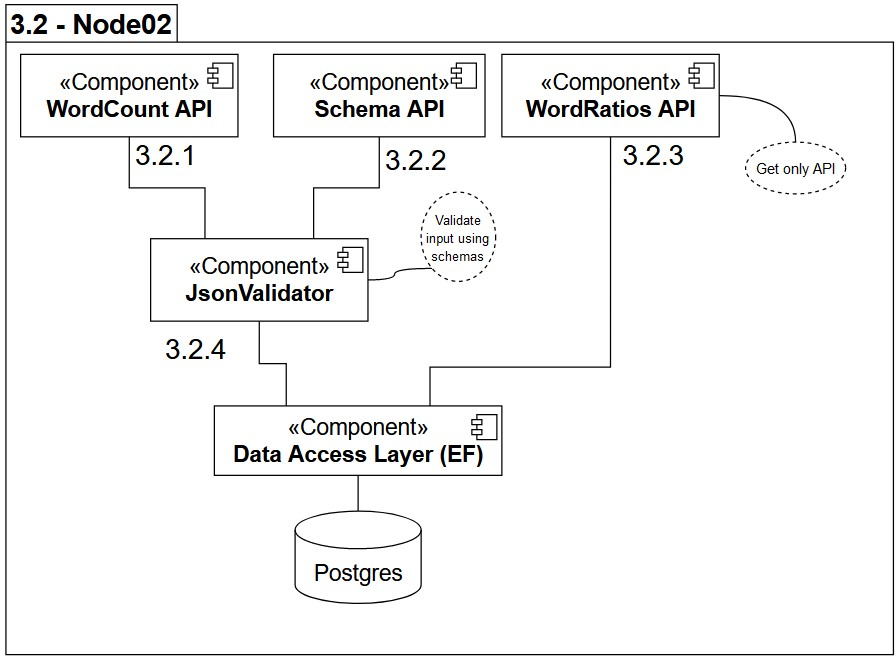
\includegraphics[width=\linewidth]{Images/Node02Pipeline.jpg}
    \caption{Node02 database access API components in sprint 3.}
    \label{Node02Sprint3}
\end{figure}

In the following sections, we will describe how the API and input validation were implemented. 
Additionally, we will cover the re-design of the database.

In order to illustrate how our layer interacts with the adjacent layers' components, we have included figure \ref{PipelineLayer2} and \ref{PipelineLayer4}.

\begin{figure}[h!]
    \centering
    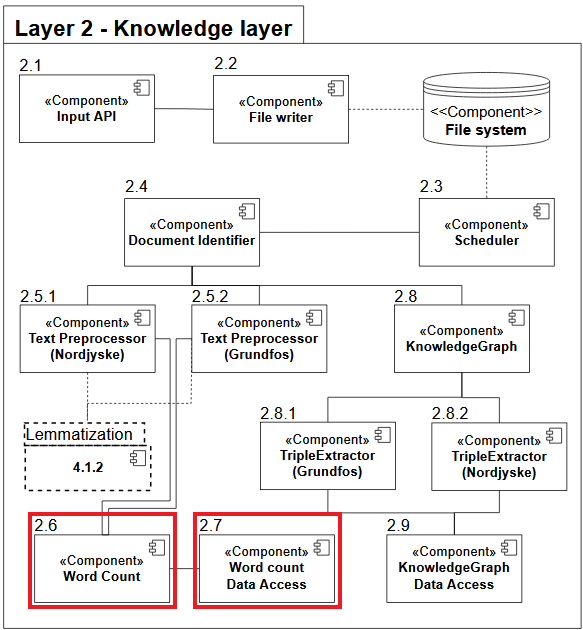
\includegraphics[scale=0.5]{Images/PipeLineLayer2.png}
    \caption{Illustration of how the knowledge layer interacts with our APIs.}
    \label{PipelineLayer2}
\end{figure}

\begin{figure}[h!]
    \centering
    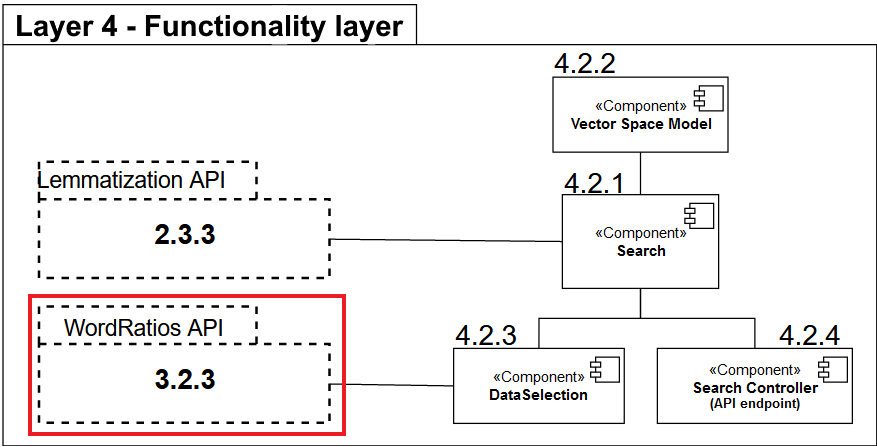
\includegraphics[scale=0.4]{Images/PipeLineLayer4SE.png}
    \caption{Illustration of how the functionality layer interacts with our APIs.}
    \label{PipelineLayer4}
\end{figure}

The respective APIs that the two adjacent layers use as part of their pipeline are highlighted in red. 

\subsubsection{WordCount}

The first route we created was the WordCount route. It is used by the knowledge layer to insert information about an article into the database. It is also used by the functionality layer to find the file path of an article.

In the controller, we implemented two methods, a \texttt{GET} and a \texttt{POST} method.
\begin{table}[h]
    \begin{tabular}{|llll|}
    \hline
    \multicolumn{4}{|c|}{\textbf{WordCount}}                                                                                 \\ \hline
    \multicolumn{1}{|l|}{Name}                 & \multicolumn{1}{l|}{Method} & \multicolumn{1}{l|}{Input}       & Response on success       \\ \hline
    \multicolumn{1}{|l|}{\texttt{GetFilepath}} & \multicolumn{1}{l|}{GET}    & \multicolumn{1}{l|}{Integer}     & Article        \\ \hline
    \multicolumn{1}{|l|}{\texttt{Post}}        & \multicolumn{1}{l|}{POST}   & \multicolumn{1}{l|}{JSON Object} & Status message \\ \hline
    \end{tabular}
\end{table}

The \texttt{GET} method called \texttt{GetFilepath} takes an integer "id" as an argument and finds an article in the database with the given "id" and returns the articles \texttt{filePath} as a \texttt{JsonResult} if it exists, otherwise an error is sent back.
This method can be seen in code snippet \ref{lst:GetFilepathMethod}.

\begin{lstlisting}[language=CSharp, caption={The \texttt{GetFilepath} method.}, label={lst:GetFilepathMethod}]
[HttpGet]
[Route("/[controller]/filelist/{id:int}")]
public IActionResult GetFilepath(long id)
{
    try
    {
        string filePath = databaseContext.Articles
          .First(e => e.Id == id).FilePath;
        return new JsonResult(new FileIdResponse(filePath));
    }
    catch (Exception)
    {
        return BadRequest($"No entity with ID {id} exists");
    }
}
\end{lstlisting}

In WordCount, we also implemented a \texttt{POST} method called \texttt{Post}, which takes a JSON object from the HTTP body as a parameter that should correspond to an array of articles. 
This method is shown in code snippet \ref{lst:POSTMethod}.

\begin{lstlisting}[language=CSharp, caption={The \texttt{POST} method.}, label={lst:POSTMethod}]
[HttpPost]
public IActionResult Post([FromBody] JsonElement jsonElement)
{
    JsonSchema? schema = databaseContext.JsonSchemas
      .First(s => s.SchemaName == WordCountSchemaName);
    string jsonInput = jsonElement.GetRawText();

    if (schema == null)
    {
        return StatusCode(500, 
          $"\"{WordCountSchemaName}\" schema does not exist.");
    }

    // Get schema and use for validating
    if (!new JsonValidator<ArticleJsonModel[]>(schema.JsonString)
      .IsValid(jsonInput, out ArticleJsonModel[] jsonArticles))
    {
        return BadRequest("Wrong body syntax, does not follow schema.");
    }

    IEnumerable<Article> result = RemoveDuplicates(jsonArticles,
      out StringBuilder message);

    // Insert article
    IEnumerable<Article> enumerable = result as Article[] 
      ?? result.ToArray();

    databaseContext.Articles.AddRange(enumerable);
    databaseContext.SaveChanges();

    return Ok(message.ToString());
}
\end{lstlisting}

The JSON object should be valid according to a JSON schema stored in the database. The schema is used to determine whether the required format of the received JSON object is correct. If the JSON object does not fit the schema, an error message is sent back. 
We then check if any of the articles already exist in the database.
In case of duplicates, the duplicate is removed from the JSON object and a message is added to the response that the article already exists. 
The remaining articles can then be inserted into the database, and a status message is returned with the potential duplicate article names. 
 
\subsubsection{WordRatio}\label{WordRatioCrud}
The WordRatio route is used by the functionality layer to fetch specific data from the database.
As WordRatio is a view (see appendix \ref{Appendix_WordRatioOld}), the route cannot be used to store new data. 
The primary purpose of WordRatio is to check how many times a given word occurs in an article.
WordRatio consists of one \texttt{GET} method with an optional parameter. 
\begin{table}[h]
    \begin{tabular}{|llll|}
    \hline
    \multicolumn{4}{|c|}{WordRatio}                                                                            \\ \hline
    \multicolumn{1}{|l|}{Name} & \multicolumn{1}{l|}{Method} & \multicolumn{1}{l|}{Input} & Response on success \\ \hline
    \multicolumn{1}{|l|}{GetMatches} &
      \multicolumn{1}{l|}{GET} &
      \multicolumn{1}{l|}{\begin{tabular}[c]{@{}l@{}}terms (string{[}{]}), \\ sources (string{[}{]})\end{tabular}} &
      \begin{tabular}[c]{@{}l@{}}WordRatio for all articles \\ from source with term\end{tabular} \\ \hline
    \multicolumn{1}{|l|}{GetMatches} &
      \multicolumn{1}{l|}{GET} &
      \multicolumn{1}{l|}{terms (string {[}{]})} &
      \begin{tabular}[c]{@{}l@{}}WordRatio for all articles\\  with term\end{tabular} \\ \hline
    \end{tabular}
\end{table}

The \texttt{GetMatches} method is used to query one or more specific words on the WordRatio table.
One may provide one or more sources in which to search for the specified words.
If no sources are provided, the database searches for the given words in all sources.

\subsubsection{Schema}
The last route we implemented in this iteration is the Schema route, which is used to post and retrieve a JSON schema from the database. These are later used to verify JSON objects as input in other endpoints. 
This schema consists of two \texttt{GET} methods and a single \texttt{POST} method.
By creating a route for fetching the validation schemas, we enable easy validation and a common understanding of the structure of input data from the knowledge layer.
\begin{table}[h]
    \begin{tabular}{|llll|}
    \hline
    \multicolumn{4}{|c|}{\textbf{Schema}}                                                                                                     \\ \hline
    \multicolumn{1}{|l|}{Name}                     & \multicolumn{1}{l|}{Method} & \multicolumn{1}{l|}{Input}               & Response on success \\ \hline
    \multicolumn{1}{|l|}{\texttt{GetSchema}}       & \multicolumn{1}{l|}{GET}    & \multicolumn{1}{l|}{Schema name (string)} & JSON schema         \\ \hline
    \multicolumn{1}{|l|}{\texttt{GetAllSchemas}}   & \multicolumn{1}{l|}{GET}    & \multicolumn{1}{l|}{None}                & All JSON schemas    \\ \hline
    \multicolumn{1}{|l|}{\texttt{PostJSONSchemas}} & \multicolumn{1}{l|}{POST}   & \multicolumn{1}{l|}{JSON Schema}         & Status message      \\ \hline
    \end{tabular}
\end{table}

The first \texttt{GET} method is called \texttt{GetSchema} which takes a schema name as its input and returns a JSON schema with the given name if it exists. 

The second \texttt{GET} method is called GetAllSchemas which takes no input and returns all stored JSON schemas. 

The last method is a \texttt{POST} method called \texttt{PostJSONSchema}, which takes a JSON schema as its input and inserts it into the database.
The body of the post request must consist of two fields - the schema name, which is its primary key in the database, and the schema content itself. Before the schema is inserted in the database, it is checked if it is a duplicate. If that is the case, an error message will be sent in response.
A schema gets stored in the database in the format known as \texttt{jsonb}, or JSON binary, which is a built-in type provided by \postgres{}.
This format is used to store a JSON object as binary, which seems to be more efficient than the regular \texttt{json} type\cite{FasterOperationsJSONB2017}.